\begin{ParaColumn}[\bisection*{State-Dependent Elastoplasticity Model: Critical State Theory}{状态相关的弹塑性模型:临界状态理论}]
    
    The state parameter $\psi$ \citep{Been1985}, which represents the difference of current void ratio $e$ and the void ratio $e_c$ at the critical state in the same mean pressure, can be used to determine the state of soil

    \switchcolumn

    状态参数$\psi$ \citep{Been1985}表示在相同平均压力下临界状态下当前空隙率$e$和空隙率$e_c$之差,可用于确定土体状态

    \CrossColumnText{
        \begin{align}
            \psi=e-e_{c}
        \end{align}
    }
    \switchcolumn*

    \noindent
    The void ratio ec at the critical state line depends on the mean pressure; it can be defined by \citep{Yang2004}

    \switchcolumn

    \noindent
    临界状态线处的空隙率$e_c$取决于平均压力。 它可以定义为\citep{Yang2004}

    \CrossColumnText{
        \begin{align}
            e_{c}=e_{c 0}-\lambda_{c}\left(\frac{p}{p_{a t}}\right)^{\xi}
        \end{align}
    }
    \switchcolumn*

    \noindent
    where $p_{a t}=101.3 \mathrm{kPa}$ = atmospheric pressure; and $e_{c 0}, \lambda_{c},$ and $\xi=$ material parameters that are used to determine the critical state line in the $e, p$-plane.

    \switchcolumn

    \noindent
    其中$p_{a t}=101.3 \mathrm{kPa}$为大气压力;$e_{c 0}, \lambda_{c},$和$\xi=$为材料参数,这些材料参数用于确定$e,p$平面中的临界状态线。

    \switchcolumn*

    In \enautoref{figure:1}, the state parameter $\psi$ clearly shows the state of the sand; a negative value indicates dilative state and a positive value indicates contractive state. It should be noted that, in an undrained case, the total volumetric strain always keeps constant, and the attainment of the state parameter to the critical state is caused by the changes in the effective mean pressure.

    \switchcolumn

    在\cnautoref{figure:1}中,状态参数$\psi$清楚地显示了砂土的状态。 负值表示扩张状态,正值表示收缩状态。 应该注意的是,在不排水的情况下,总体积应变始终保持恒定,并且状态参数达到临界状态是由有效平均压力的变化引起的。

    \CrossColumnText{
        \begin{figure}[htb]
    \centering
    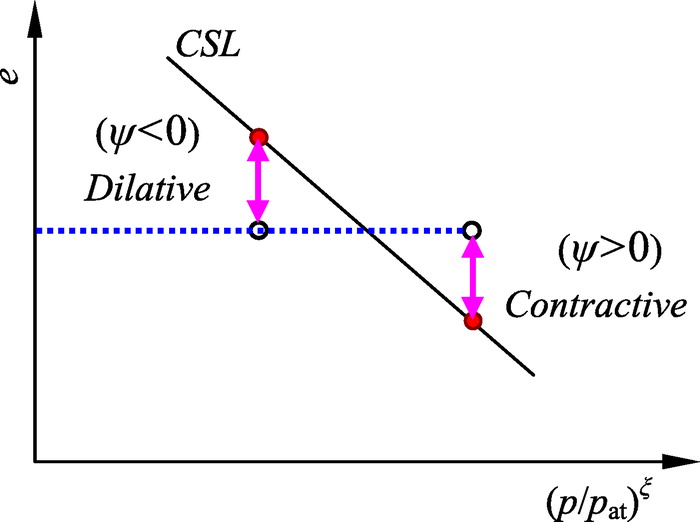
\includegraphics[width=.5\textwidth]{figures/figure1.jpg}
    \bicaption{Critical state line in $e-\left(p / p_{a t}\right)^{\xi}$ plane}{$e-\left(p / p_{a t}\right)^{\xi}$平面的临界状态线}
    \label{figure:1}
\end{figure}
    }

\end{ParaColumn}